\documentclass{article}
\usepackage{graphicx}
\usepackage{float}
\usepackage{subfig}
\usepackage{amsmath}

\begin{document}

\title{My Homework 2}
\author{Mauro Patimo}
\date{\today}

\maketitle

\section{Ex 1}
\begin{figure}[H]
    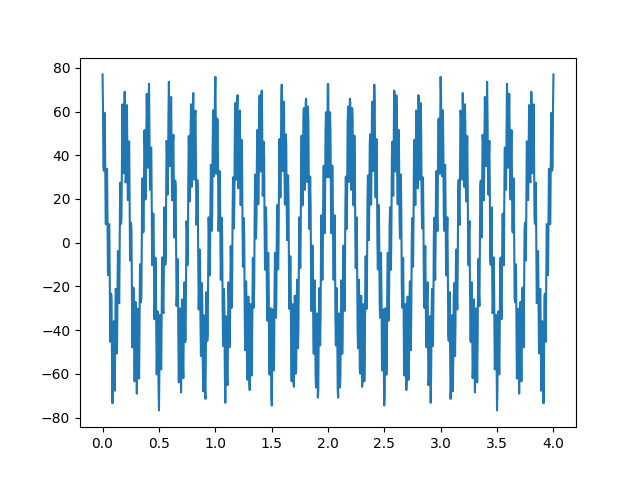
\includegraphics[width=\textwidth]{HW2_1.png}
    \caption{Initial signal}
\end{figure}
\begin{figure}[H]
    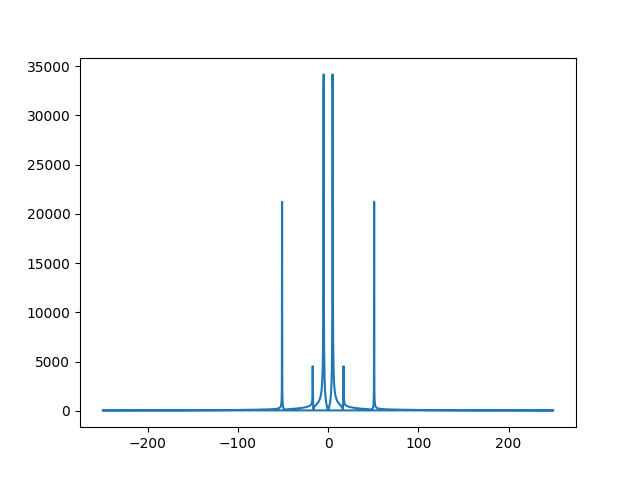
\includegraphics[width=\textwidth]{HW2_1frequency.png}
    \caption{Fourier Transform of the initial signal}
\end{figure}
The number of points $N_P$ is useful for the discretization of our function, to allow computers to work with it. It is important to have a good number of points to avoid the discretization error. In fact, if the number of points is too low, the signal will be discretized with a low resolution, and the fourier transform will not be able to capture the true frequency of the signal, due to a possible aliasing effect. \\
$f_s$ is the sampling frequency, and it is important for the definition of the time axis. It is important to have a good sampling frequency to avoid the aliasing effect. Where the frequency ($1/f_s$) is lower then one the frequency of the signal, and therefore it is not able to capture the correct frequency of the signal. \\
$T_f$ is the period of time over which we are taking values of our signal, and it is important for the definition of the time axis. It is important to have a good final time (usually the longer the better for frequency analysis and the shorter the better for time analysis) to avoid the truncation of the signal. In fact, if the final time is too short, the signal will be truncated and the true frequency of the signal will not be captured, because the fourier transform will not be able to capture an entire period. \\
\section{Ex 2}
\begin{figure}[H]
    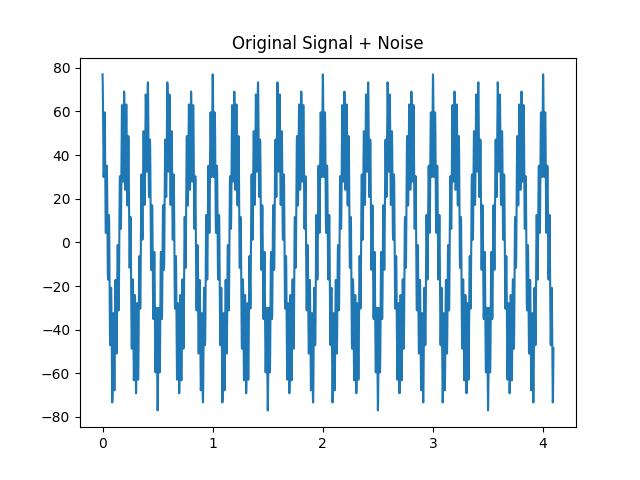
\includegraphics[width=\textwidth]{HW2_2time.png}
    \caption{Signal with noise}
\end{figure}
\begin{figure}[H]
    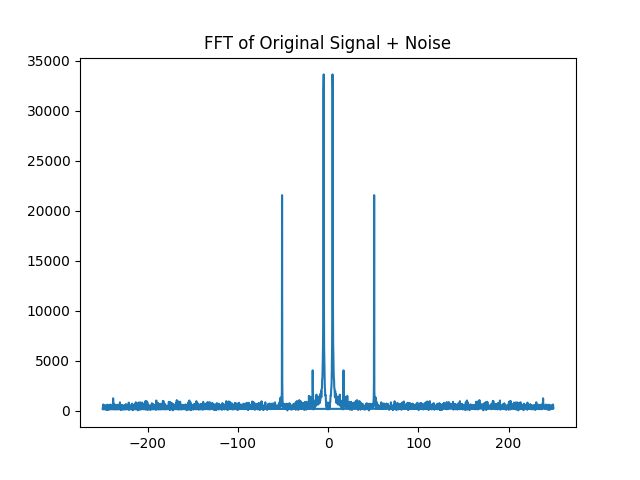
\includegraphics[width=\textwidth]{HW2_2freq.png}
    \caption{Fourier Transform of the noisy signal}
\end{figure}
\begin{figure}[H]
    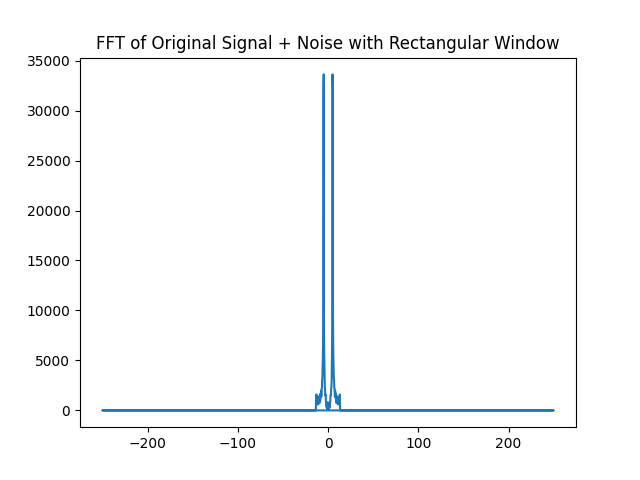
\includegraphics[width=\textwidth]{HW2_2freq_55points.png}
    \caption{Filtered noisy signal}
\end{figure}
This is the signal after passing under the filter. What the filter does it to keep the frequencies lower than a certain threshold. As visible only the 5Hz is kept. 
A lot of the noise has been however removed. \\
\begin{figure}[H]
    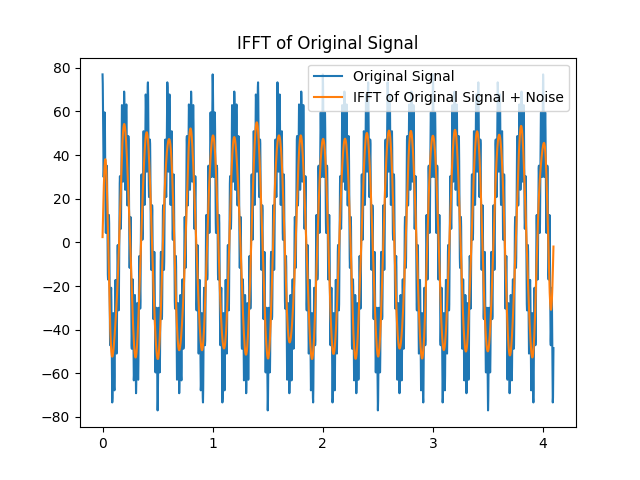
\includegraphics[width=\textwidth]{HW2_2IFFT_55points.png}
    \caption{Filtered noisy signal}
\end{figure}
The signal is now a lot cleaner, but it also has lost of a lot of information. The main shape remained the same, because the frequency with the greatest amplitude has been kept, but it doesn't match the real signal perfectly. 
We can match the real signal perfectly only if we keep all the frequencies, but then we would also keep all the noise. So we can increase the size of our rectangular function to include all the main frequencies and get rid of some noise that has very high frequencies to match match the original signal better. \\
\section{Ex 3}
\begin{figure}[H]
    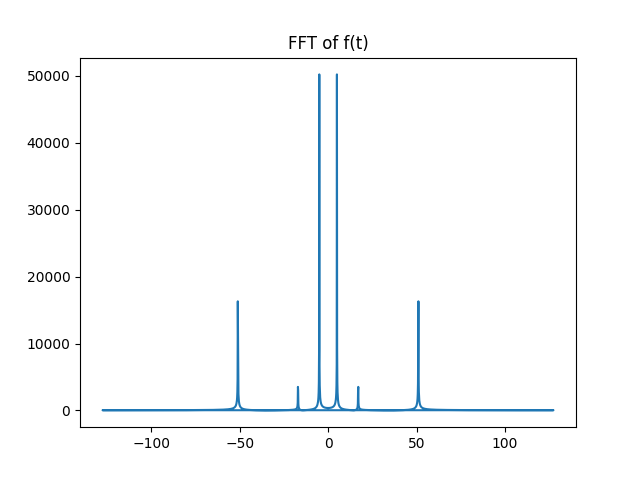
\includegraphics[width=\textwidth]{HW2_3a.png}
    \caption{Fourier Transform of initial signal}
\end{figure}
\begin{figure}[H]
    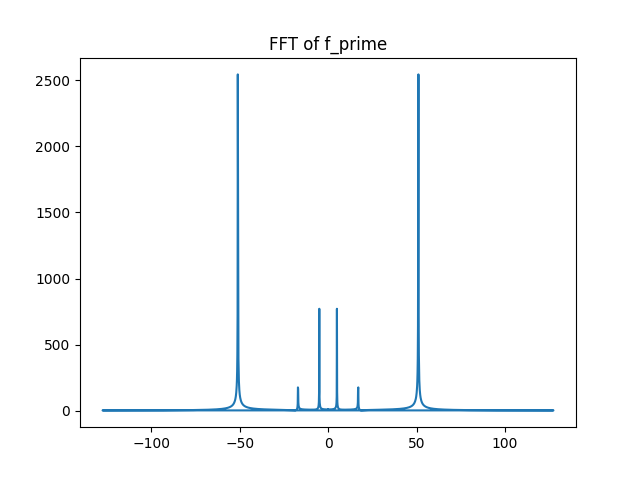
\includegraphics[width=\textwidth]{HW2_3_FFT_f'.png}
    \caption{Fourier Transform of the derivative of initial signal}
\end{figure}
\begin{figure}[H]
    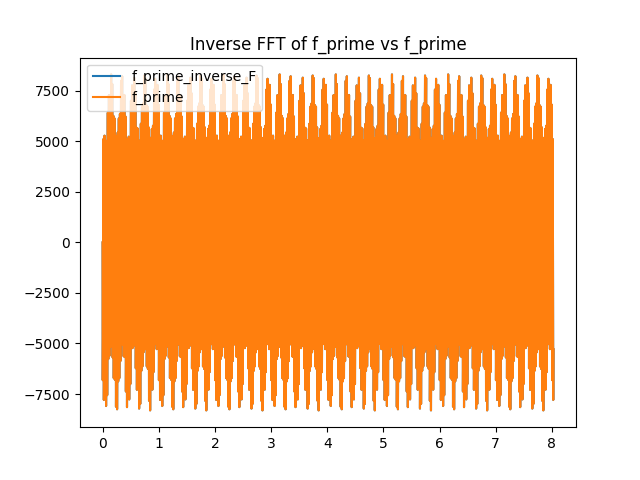
\includegraphics[width=\textwidth]{HW2_3d.png}
    \caption{Two signal superimposed}
\end{figure}
\section*{Ex 4}
\begin{figure}[H]
    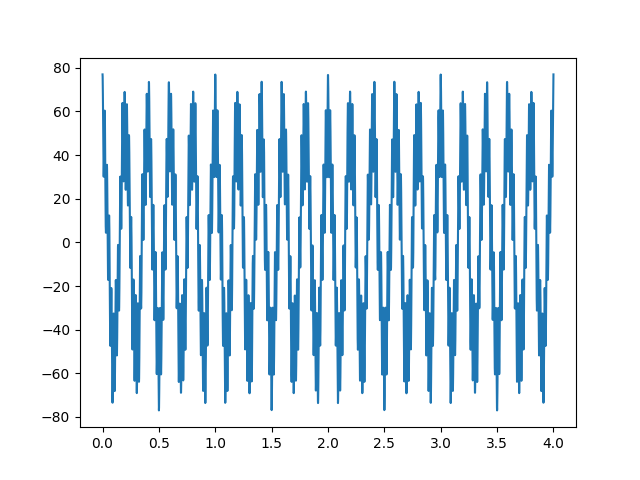
\includegraphics[width=\textwidth]{4a.png}
\end{figure}
Magnitude plot of the signal.
\begin{figure}[H]
    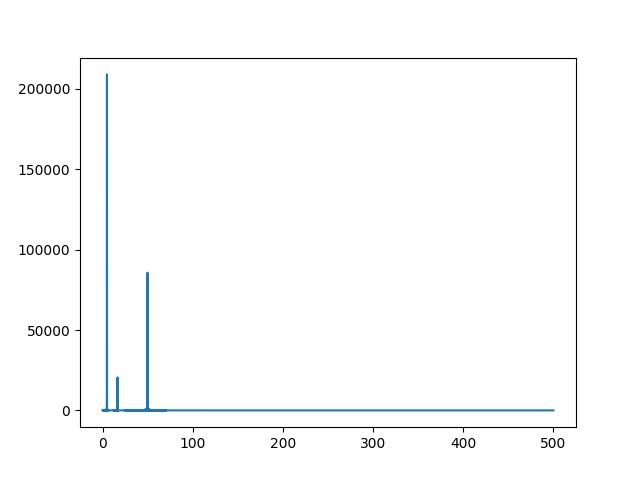
\includegraphics[width=\textwidth]{4b.png}
\end{figure}
FFT of the signal.
\begin{figure}[H]
    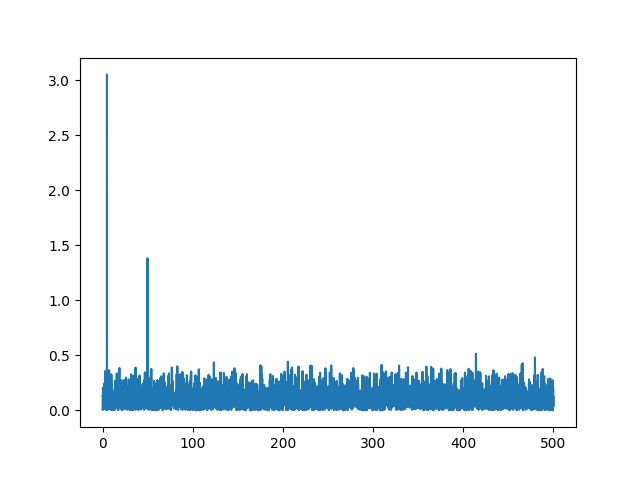
\includegraphics[width=\textwidth]{4d.png}
\end{figure}
FFT of the compressed signal.
\begin{figure}[H]
    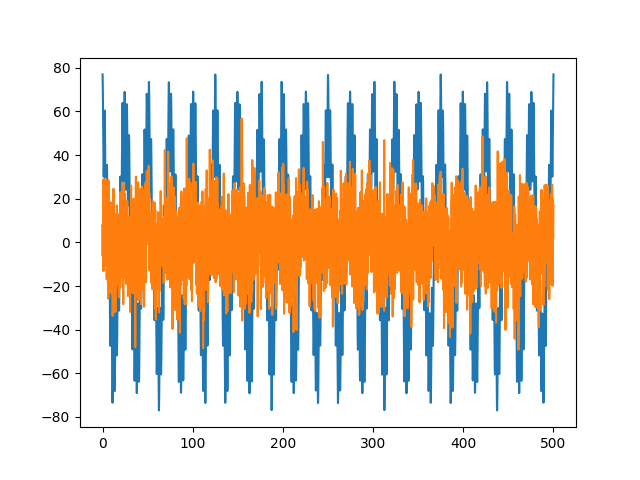
\includegraphics[width=\textwidth]{4e.png}
\end{figure}
Compressed vs original signal. The compressed signal is similar in frequencies as the original one, but its mangitudes are much lower. This is due to the least square method, that tries to minimize the error between the original and the compressed signal.
\begin{figure}[H]
    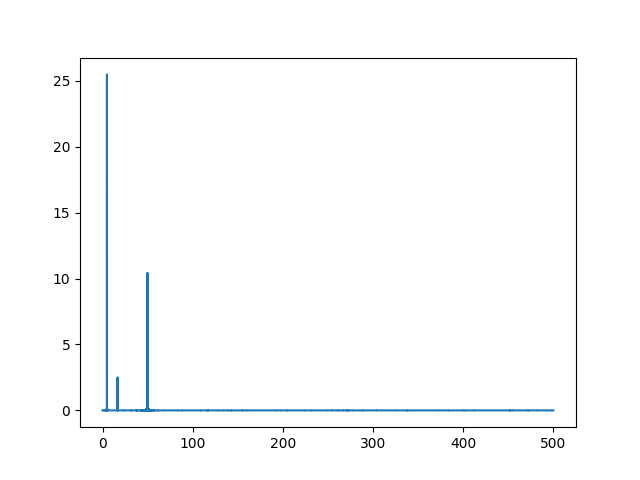
\includegraphics[width=\textwidth]{4f.png}
\end{figure}
Frequency plot of the reconstructed compressed signal.
\section*{Ex 5}
\begin{figure}[H]
    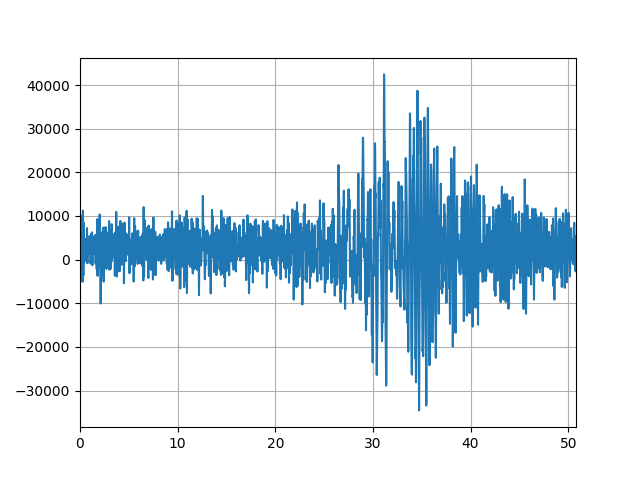
\includegraphics[width=\textwidth]{Ex 5a.1.png}
    \caption{Earthquake}
\end{figure}
\begin{figure}[H]
    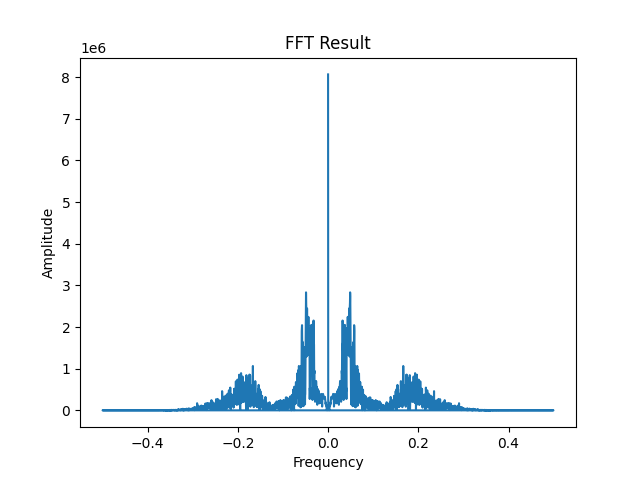
\includegraphics[width=\textwidth]{Ex 5a.2.png}
    \caption{FFT}
\end{figure}
\subsection*{C}
\begin{figure}
    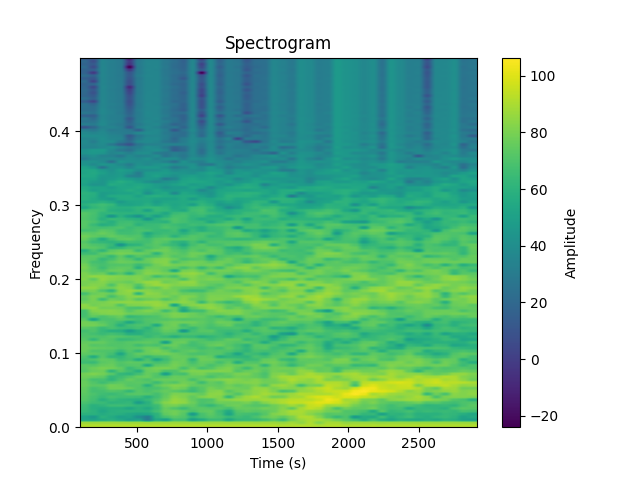
\includegraphics[width=\textwidth]{Ex 5c.png}
    \caption{Spectogram}
\end{figure}
The Earthquake seems to have a frequency of 0.5Hz, and it is visible in the spectogram, with the a peak in magnitude starting at around 1700s. This is proven in the mangitude plot as the mangitude remains the same (which is probably noise) and peaks in magntidue then. \\
\end{document}
